\documentclass{notes}

\title{Lecture Notes on Radio Frequency Electronic Circuits}
\author{\href{https://github.com/LittleYe233}{LittleYe233} \textit{a.k.a.} Zhifan Ye <\href{mailto:littleye233@gmail.com}{littleye233@gmail.com}>}
% See: https://tex.stackexchange.com/a/142973
\datemodified{\DTMdate{2023-2-23}}
\version{1.1.0}

\tikzstyle{normal} = [
    rectangle,
    rounded corners,
    minimum width=2cm,
    minimum height=1cm,
    text centered,
    draw=black
]

\begin{document}

\maketitle
\tableofcontents
\newpage

\section*{课程信息} \label{课程信息}
\addcontentsline{toc}{section}{课程信息}

\subsection{地点}
\textbf{教室:} T5204 \par
\textbf{座位:} 6 排 4 列

\subsection{授课教师}
王凯旭 <\href{mailto:wangkaixu@hit.edu.cn}{wangkaixu@hit.edu.cn}>

\subsection{分数构成}
\begin{itemize}
    \item 平时成绩 (30\%)
          \begin{itemize}
              \item 作业 (5\%)
              \item 课堂表现 (5\%)
              \item 随堂作业或测验 (20\%)
          \end{itemize}
    \item 期末考试 (70\%)
\end{itemize}

\section{绪论} \label{绪论}
\subsection{无线电信号传输原理}
\subsubsection{传输信号的基本方法}
\begin{figure}[ht]
    \centering
    \begin{tikzpicture}
        \node (1) [normal] {信号源};
        \node (2) [normal, right=of 1] {发送设备};
        \node (3) [normal, right=of 2] {传输信道};
        \node (4) [normal, right=of 3] {接收设备};
        \node (5) [normal, right=of 4] {收信装置};

        \draw [-latex] (1) edge (2)
        (2) edge (3)
        (3) edge (4)
        (4) edge (5);
    \end{tikzpicture}
    \caption{通信系统组成框图}
\end{figure}

\begin{itemize}
    \item \textbf{发送设备}\quad 转换为适合传输的信号.
    \item \textbf{收信装置}\quad 扬声器, 等.
\end{itemize}

\subsubsection{无线电信号的产生与发射}
\begin{figure}[ht]
    \centering
    \begin{tikzpicture}
        \node (1) [normal] {高频振荡};
        \node (2) [normal, right=of 1] {倍频};
        \node (3) [normal, right=of 2] {高频放大};
        \node (4) [normal, right=of 3] {调制};
        \node (5) [normal, below=of 2] {音频源};
        \node (6) [normal, right=of 5] {音频放大};
        \node (7) [right=1.5cm of 4] {};

        \draw [-latex] (1) -- (2) node [midway, above] {缓冲};
        \draw [-latex] (2) edge (3)
        (3) edge (4)
        (5) edge (6)
        (6) -| (4);
        \draw [-latex] (4) -- (7) node [midway, above] {传输线};
    \end{tikzpicture}
    \caption{无线电发射机方框图}
\end{figure}

\textbf{调制}\quad 将声音电流加在高频电流上.
\begin{itemize}
    \item \textbf{分类}\quad 调幅 (AM, 高频振幅变化所形成的包络波形即为原信号波形), 调频 (FM), 调相 (PM).
    \item \textbf{原因}
          \begin{itemize}
              \item 传输低频信号需要更庞大的天线;
              \item 减少干扰, 提高信道复用率 (将信号放大到不同的频段).
          \end{itemize}
\end{itemize}

\subsubsection{无线电信号的接收}
\textbf{接收设备}要求尽可能减少失真.

\begin{figure}[ht]
    \centering
    \begin{tikzpicture}
        \node (1) [] {};
        \node (2) [normal, right=1.5cm of 1] {选择性电路};
        \node (3) [normal, right=of 2] {检波};
        \node (4) [normal, right=of 3] {发声装置};

        \draw [-latex] (1) -- (2) node [midway, above] {传输线};
        \draw [-latex] (2) edge (3)
        (3) edge (4);
    \end{tikzpicture}
    \caption{最简单的接收机方框图}
\end{figure}

\begin{figure}[ht]
    \centering
    \begin{tikzpicture}
        \node (1) [] {};
        \node (2) [normal, right=1.5cm of 1] {高频放大};
        \node (3) [normal, right=of 2] {混频};
        \node (4) [normal, right=of 3] {中频放大};
        \node (5) [normal, right=of 4] {检波};
        \node (6) [normal, right=of 5] {低频放大};
        \node (7) [normal, below=of 3] {本地振荡};

        \draw [-latex] (1) -- (2) node [midway, above] {传输线};
        \draw [-latex] (2) edge (3)
        (3) edge (4)
        (4) edge (5)
        (5) edge (6)
        (7) edge (3);
    \end{tikzpicture}
    \caption{超外差式接收机方框图}
\end{figure}

\subsection{通信的传输媒质}
\begin{itemize}
    \item 有线通信
          \begin{itemize}
              \item 双线对电缆 (双绞线; 频率低)
              \item 同轴电缆
              \item 光纤 (频率高, 衰减小)
          \end{itemize}
    \item 无线通信
          \begin{itemize}
              \item 地波
                    \begin{itemize}
                        \item 地面波 (电磁波沿地面绕射传输; 传播距离近, 频率低)
                        \item 空间波 (由直射波, 反射波组成; 视距范围内)
                    \end{itemize}
              \item 天波 (通过空中电离层的折射反射传播, 穿透电离层, 更高频率会携带水蒸气)
          \end{itemize}
\end{itemize}

\section{选频网络}
\begin{itemize}
    \item 振荡回路 (由 L, C 组成)
          \begin{itemize}
              \item 单振荡回路
              \item 耦合振荡回路
          \end{itemize}
    \item 滤波器
          \begin{itemize}
              \item LC 集中滤波器
              \item 石英晶体滤波器
              \item 陶瓷滤波器
              \item 声表面波滤波器
          \end{itemize}
\end{itemize}

\subsection{串联谐振回路}
\subsubsection{基本原理}
\begin{figure}[ht]
    \centering
    \begin{tikzpicture}[circuit ee IEC, x=3cm, y=2cm, semithick, every info/.style={font=\normalsize}, large circuit symbols]
        \draw (0, 0) to [voltage source={info={$\dot{V}_s$}}] (0, 1);
        \draw (0, 1) to [inductor={info={$L$}}] (1, 1);
        \draw (1, 1) to [capacitor={info={$C$}}] (1, 0);
        \draw (1, 0) to [resistor={info={$R$}}] (0, 0);
    \end{tikzpicture}
    \caption{串联谐振回路}
\end{figure}

\textbf{阻抗}

\begin{equation}
    Z=R+\mathrm{j}\left(\omega L-\frac{1}{\omega C}\right)=|Z|e^{\mathrm{j}\varphi}.
\end{equation}

其中

\begin{equation}
    X=\left(\omega L-\frac{1}{\omega C}\right).
\end{equation}

\begin{equation}
    |Z|=\sqrt{R^2+X^2}=\sqrt{R^2+\left(\omega L-\frac{1}{\omega C}\right)^2}.
\end{equation}

\begin{equation}
    \varphi=\arctan\frac{X}{R}=\arctan\frac{\omega L-\dfrac{1}{\omega C}}{R}.
\end{equation}

\textbf{谐振条件}\quad $\omega=\omega_0=\dfrac{1}{\sqrt{LC}}$. $f_0=\dfrac{1}{2\pi\sqrt{LC}}$.

\textbf{特性阻抗}\quad 谐振时的感抗或容抗. $\rho=\sqrt{\dfrac{L}{C}}$.

\textbf{非谐振特性}

当 $\omega\neq\omega_0$ 时, $|Z|>R$.

\begin{itemize}
    \item $\omega>\omega_0$, $X>0$, 呈感性; $|\dot{V}_L|<|\dot{V}_C|$; $\varphi>0$, 电流滞后电压;
    \item $\omega<\omega_0$, $X<0$, 呈容性; $|\dot{V}_L|>|\dot{V}_C|$; $\varphi<0$, 电流超前电压.
\end{itemize}

\textbf{谐振特性}

\begin{itemize}
    \item $X=0$, $Z=R$, 呈纯阻性, $|Z|$ 达到最小值;
    \item $\varphi=0$, 电流与电压同相位;
    \item L 和 C 上的电压 $\dot{V}_{L0}$ 和 $\dot{V}_{C0}$ 大小相等, 相位相差 180°, $\dot{V}_s=\dot{V}_R$;
    \item $\dot{V}_{L0}=\mathrm{j}Q\dot{V}_s$, $\dot{V}_{C0}=-\mathrm{j}Q\dot{V}_s$, 其中 $Q=\dfrac{\omega_0L}{R}=\dfrac{1}{\omega_0CR}=\dfrac{\rho}{R}=\dfrac{1}{R}\sqrt{\dfrac{L}{C}}$ 为回路的\textbf{品质因数} ($Q$ 越高, 回路选择性越好).
\end{itemize}

\begin{figure}[ht]
    \centering
    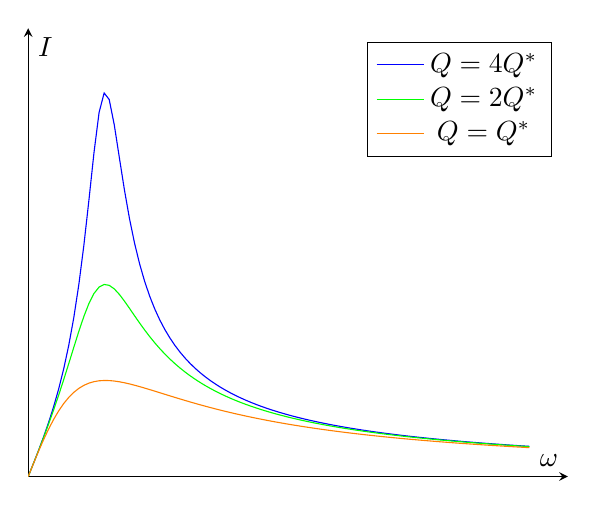
\begin{tikzpicture}
        % See: https://tex.stackexchange.com/a/569760
        \begin{axis}[
                samples=100,
                domain=0:6.5,
                xmin=0, xmax=7,
                ymin=0, ymax=7,
                axis lines=middle,
                ticks=none,
                xlabel={$\omega$},
                ylabel={$I$},
                legend pos=north east]
            \addplot [blue] {3/(sqrt(0.5^2+(\x-1/\x)^2))};
            \addplot [green] {3/(sqrt(1^2+(\x-1/\x)^2))};
            \addplot [orange] {3/(sqrt(2^2+(\x-1/\x)^2))};
            \addlegendentry{$Q=4Q^*$};
            \addlegendentry{$Q=2Q^*$};
            \addlegendentry{$Q=Q^*$};
        \end{axis};
    \end{tikzpicture}
    \caption{外加电压为常数时, $Q$ (或 $R$) 对 $I$-$\omega$ 曲线的影响 (谐振曲线)}
\end{figure}

当 $\dot{V}_s$ 保持不变时, $|\dot{I}|$ 达到最大值.

\subsubsection{串联振荡回路的谐振曲线和通频带} \label{串联振荡回路的谐振曲线和通频带}

\begin{equation}
    \frac{\dot{I}}{\dot{I}_0}=\frac{1}{1+\mathrm{j}Q\left(\dfrac{\omega}{\omega_0}-\dfrac{\omega_0}{\omega}\right)}.
\end{equation}

\begin{equation}\label{2.1.2 I/I_0}
    \frac{I}{I_0}=\frac{1}{\sqrt{1+\left(\dfrac{X}{R}\right)^2}}=\frac{1}{\sqrt{1+Q^2\left(\dfrac{\omega}{\omega_0}-\dfrac{\omega_0}{\omega}\right)^2}}.
\end{equation}

\textbf{失谐 (失调)}\quad $\Delta\omega=\omega-\omega_0$.

当 $\omega\approx\omega_0$ 时, 利用

\begin{equation*}
    \frac{\omega}{\omega_0}-\frac{\omega_0}{\omega}=\frac{\omega^2-\omega_0^2}{\omega_0\omega}=\left(\frac{\omega+\omega_0}{\omega}\right)\left(\frac{\omega-\omega_0}{\omega_0}\right)\approx 2\frac{\Delta\omega}{\omega_0},
\end{equation*}

\noindent 将 (\ref{2.1.2 I/I_0}) 改写为\textit{小量失谐}情况下通用形式的\textbf{谐振特性方程式}

\begin{equation}
    \frac{I}{I_0}\approx\frac{1}{\sqrt{1+\left(Q\dfrac{2\Delta\omega}{\omega_0}\right)^2}}=\frac{1}{\sqrt{1+\xi^2}}.
\end{equation}

\textbf{广义失谐 (一般失谐)}\quad $\xi=Q\dfrac{2\Delta\omega}{\omega_0}$.

\textbf{边界角频率 (频率)}\quad $\dfrac{I}{I_0}=\dfrac{1}{\sqrt{2}}$ 时的 $\omega_{1,2}$ ($f_{1,2}$).

此时回路损耗功率为谐振功率的一半 (半功率点). $\xi=\pm 1$.

\textbf{通频带}\quad $2\Delta\omega_{0.7}=\omega_2-\omega_1=\dfrac{\omega_0}{Q}$, $2\Delta f_{0.7}=f_2-f_1=\dfrac{f_0}{Q}$.

$Q$ 越高, 通频带越窄.

考虑信号源内阻时, 若信号源变为恒流源 ($R_s$ 和 $V_s$ 可趋于无穷大), $Q$ 降为零.

\newpage

\section*{更新日志} \label{更新日志}
\addcontentsline{toc}{section}{更新日志}
\subsection*{1.1.0 (2023-2-23)}
\begin{itemize}
    \item 增加 \ref{绪论} 至 \ref{串联振荡回路的谐振曲线和通频带} 的部分;
    \item 增加 \hyperref[更新日志]{更新日志}.
\end{itemize}

\subsection*{1.0.0 (2023-2-22)}
\begin{itemize}
    \item 增加 \hyperref[课程信息]{课程信息} 的部分.
\end{itemize}

\end{document}
